%%%%%%%%%%%%%%%%%%%%%%%%%%%%%%%%%%%%%%%%%%%%%%%%%%%%%%%%%%%%%%%%%%%%%%%%%%%%%
%%%
%%% File: utthesis2.doc, version 2.0jab, February 2002
%%%
%%% Based on: utthesis.doc, version 2.0, January 1995
%%% =============================================
%%% Copyright (c) 1995 by Dinesh Das.  All rights reserved.
%%% This file is free and can be modified or distributed as long as
%%% you meet the following conditions:
%%%
%%% (1) This copyright notice is kept intact on all modified copies.
%%% (2) If you modify this file, you MUST NOT use the original file name.
%%%
%%% This file contains a template that can be used with the package
%%% utthesis.sty and LaTeX2e to produce a thesis that meets the requirements
%%% of the Graduate School of The University of Texas at Austin.
%%%
%%% All of the commands defined by utthesis.sty have default values (see
%%% the file utthesis.sty for these values).  Thus, theoretically, you
%%% don't need to define values for any of them; you can run this file
%%% through LaTeX2e and produce an acceptable thesis, without any text.
%%% However, you probably want to set at least some of the macros (like
%%% \thesisauthor).  In that case, replace "..." with appropriate values,
%%% and uncomment the line (by removing the leading %'s).
%%%
%%%%%%%%%%%%%%%%%%%%%%%%%%%%%%%%%%%%%%%%%%%%%%%%%%%%%%%%%%%%%%%%%%%%%%%%%%%%%

\documentclass[a4paper, 12pt, oneside]{report}         %% LaTeX2e document.
\usepackage {tcdthesis}              %% Preamble.

%%For loading graphic files
\usepackage{graphicx}
%% subfigure
\usepackage{caption}
\usepackage{subcaption}
%% bookmark
\usepackage{hyperref}
%% url
\usepackage{url}
\usepackage{textgreek}
%% image path
\graphicspath{{../img/CGVC2015/}{../img/EuroVis2015/}{../img/TransferReport/}{../img/EurasiaGraphics2014/images/}{../img/EurasiaGraphics2014/images1/}{../img/EurasiaGraphics2014/images2/}{../img/EurasiaGraphics2014/images3/}{../img/EurasiaGraphics2014/images4/}}
\usepackage{lmodern} %Type1-font for non-english texts and characters

%% Math Packages %%%%%%%%%%%%%%%%%%%%%%%%%%%%%%%%%%%%%%%%%%%%
\usepackage{amsmath}
\usepackage{amsthm}
\usepackage{amsfonts}

% other packages
\usepackage{cite}
\usepackage{braket}
\newcommand\addtag{\refstepcounter{equation}\tag{\theequation}}

% \mastersthesis                     %% Uncomment one of these; if you don't
\phdthesis                         %% use either, the default is \phdthesis.

%\thesisdraft                       %% Uncomment this if you want a draft
                                     %% version; this will print a timestamp
                                     %% on each page of your thesis.

\leftchapter                       %% Uncomment one of these if you want
%\centerchapter                      %% left-justified, centered or
% \rightchapter                      %% right-justified chapter headings.
                                     %% Chapter headings includes the
                                     %% Contents, Acknowledgments, Lists
                                     %% of Tables and Figures and the Vita.
                                     %% The default is \centerchapter.

% \singlespace                       %% Uncomment one of these if you want
\oneandhalfspace                   %% single-spacing, space-and-a-half
% \doublespace                       %% or double-spacing; the default is
                                     %% \oneandhalfspace, which is the
                                     %% minimum spacing accepted by the
                                     %% Graduate School.

\renewcommand{\thesisauthor}{Shengzhou Luo}            %% Your official UT name.
\renewcommand{\thesismonth}{August}                  %% Your month of graduation.
\renewcommand{\thesisyear}{2015}                      %% Your year of graduation.
\renewcommand{\thesistitle}{Information-Guided Transfer Function Optimization for Volume Visualization}            %% The title of your thesis; use mixed-case.
\renewcommand{\thesisauthorpreviousdegrees}{MSc}  %% Your previous degrees, abbreviated; separate multiple degrees by commas.
\renewcommand{\thesissupervisor}{John Dingliana}      %% Your thesis supervisor; use mixed-case and don't use any titles or degrees.
% \renewcommand{\thesiscosupervisor}{}                %% Your PhD. thesis co-supervisor; if any.

% \renewcommand{\thesiscommitteemembera}{}
% \renewcommand{\thesiscommitteememberb}{}
% \renewcommand{\thesiscommitteememberc}{}
% \renewcommand{\thesiscommitteememberd}{}
% \renewcommand{\thesiscommitteemembere}{}
% \renewcommand{\thesiscommitteememberf}{}
% \renewcommand{\thesiscommitteememberg}{}
% \renewcommand{\thesiscommitteememberh}{}
% \renewcommand{\thesiscommitteememberi}{}

\renewcommand{\thesisauthoraddress}{Dublin, Ireland}

\renewcommand{\thesisdedication}{}     %% Your dedication, if you have one; use "\\" for linebreaks.


%%%%%%%%%%%%%%%%%%%%%%%%%%%%%%%%%%%%%%%%%%%%%%%%%%%%%%%%%%%%%%%%%%%%%%%%%%%%%
%%%
%%% The following commands are all optional, but useful if your requirements
%%% are different from the default values in utthesis.sty.  To use them,
%%% simply uncomment (remove the leading %) the line(s).

% \renewcommand{\thesiscommitteesize}{...}
                                     %% Uncomment this only if your thesis
                                     %% committee does NOT have 5 members
                                     %% for \phdthesis or 2 for \mastersthesis.
                                     %% Replace the "..." with the correct
                                     %% number of members.

% \renewcommand{\thesisdegree}{...}  %% Uncomment this only if your thesis
                                     %% degree is NOT "DOCTOR OF PHILOSOPHY"
                                     %% for \phdthesis or "MASTER OF ARTS"
                                     %% for \mastersthesis.  Provide the
                                     %% correct FULL OFFICIAL name of
                                     %% the degree.

% \renewcommand{\thesisdegreeabbreviation}{...}
                                     %% Use this if you also use the above
                                     %% command; provide the OFFICIAL
                                     %% abbreviation of your thesis degree.

% \renewcommand{\thesistype}{...}    %% Use this ONLY if your thesis type
                                     %% is NOT "Dissertation" for \phdthesis
                                     %% or "Thesis" for \mastersthesis.
                                     %% Provide the OFFICIAL type of the
                                     %% thesis; use mixed-case.

% \renewcommand{\thesistypist}{...}  %% Use this to specify the name of
                                     %% the thesis typist if it is anything
                                     %% other than "the author".

%%%
%%%%%%%%%%%%%%%%%%%%%%%%%%%%%%%%%%%%%%%%%%%%%%%%%%%%%%%%%%%%%%%%%%%%%%%%%%%%%



\begin{document}                                  %% BEGIN THE DOCUMENT

%\thesistitlepage                                  %% Generate the title page.

%\thesisdeclarationpage				  %% Generate the declaration page.

%\thesispermissionpage				  %% Generate the copyright permission page

%\thesisdedicationpage                             %% Generate the dedication page.

%\begin{thesisacknowledgments}                     %% Use this to write your
%...ACKNOWLEDGMENTS...                          %% acknowledgments; it can be anything
%\end{thesisacknowledgments}                       %% allowed in LaTeX2e par-mode.

%\begin{thesisabstract}
%Volume data is widely used in scientific and medical research, and volume visualization has been proven to be an effective and flexible method for visualizing complex structures. This thesis examines the methods for exploring of volume data by optimization of visualization parameters and through the use of focus and context visualization techniques by selectively enhancing important parts of the data sets.
%
%
%%Volume data is widely used in scientific and medical research, and volume visualization has been proven to be an effective and flexible method for visualizing complex structures within volume data.
%%In recent years, volume visualization has received increasing attention in the analysis of dynamics and evolution of phenomena in a variety of application domains, including medicine, meteorology, astrophysics and engineering.
%%However, the size and complexity of the parameter space controlling the rendering process makes it challenging to generate an informative rendering.
%%In particular, the specification of the transfer function (which is a mapping from data values to visual properties ) is frequently a time-consuming and unintuitive task.
%
%%We propose a novel approach to optimise the transfer functions in volume visualization by exploiting the information inherent within the volume data.
%%We hypothesise that the importance of voxels (sample values in volume data) are associated with their information content. Therefore, the transfer functions of volume visualization can be optimized based on the information within the data sets. The user's interests are also taken into account in this approach through interactive input (such as user-selected regions).
%%This optimization approach reduces the occlusion in the resulting images, and thus improves the perception of structures in the rendered images.
%%In particular we believe our approach will be useful in visualizing time-varying details by adaptively optimizing the visualization parameters according to the changes over time.
%%
%%NPR techniques are effective forms of abstraction and they have proven useful in expressing features that are difficult to display using realistic depiction of scenes and objects.
%%We explore the use of NPR techniques to enhance the perception of structures within the volume data by highlighting important details and simplifying less important details, as well as depicting the dynamic aspects of time-varying volume data.
%%We argue that the combination of standard volume visualization and NPR techniques can provide opportunities to deliver meaningful visualization and assist users in accomplishing their underlying problems efficiently.
%%
%
%
%
%Volume visualization is a powerful technique for depicting layered structures in 3D volume data sets. However, it is a major challenge to obtain clear visualizations of a volume with layers clearly revealed.
%In particular, the specification of the transfer function is frequently a time-consuming and unintuitive task in volume rendering.
%We describe a global optimization and two user-driven refinement methods for modulating transfer functions in order to assist the exploration of volume data.
%This optimization is dependent on the distribution of scalar values of the volume data set and is designed to reduce general occlusion and improve the clarity of layers of structures in the resulting images.
%The user can explore a volume by interactively specifying different priority intensity ranges and observe which layers of structures are revealed. In addition we show how the technique can be applied for time-varying volume data sets by adaptively refining the transfer function based on the histogram of each time-step. 
%Experimental results on various data sets are presented to demonstrate the effectiveness of our method.
%
%
%Volume visualization has been widely used to depict complicated 3D structures in volume data sets.
%However, obtaining clear visualization of the features of interest in a volume is still a major challenge.
%The clarity of features depends on the transfer function, the viewpoint and the spatial distribution of features in the volume data set.
%We propose visibility-weighted saliency as a measure of visual saliency of features in volume rendered images, in order to assist users in choosing suitable viewpoints and designing effective transfer functions to visualize the features of interest. Visibility-weighted saliency is based on a computational measure of perceptual importance of voxels and the visibility of features in volume rendered images.
%The effectiveness of this scheme is demonstrated by test results on two volume data sets.
%
%
%Time-varying volume data is used in many areas of science and engineering. However visualizations of such data are not easy for users to visually process due to the amount of information that can be presented simultaneously. We propose a novel visualization approach which modulates focus, emphasizing important information, by adjusting saturation and brightness of voxels based on an importance measure derived from temporal and multivariate information. By conducting a voxel-wise analysis of a number of consecutive frames, we acquire a volatility measure of each voxel. We then use intensity, volatility and additional multivariate information to determine opacity, saturation and brightness of the voxels. The method was tested in visualizing a multivariate hurricane data set. The results suggest that our approach can give the user a deeper understanding of the data by presenting multivariate information variables in one self-contained visualization.
%\end{thesisabstract}

%\tableofcontents                                  %% Generate table of contents.
%\listoftables                                     %% Uncomment this to generate list of tables.
%\listoffigures                                    %% Uncomment this to generate list of figures.

%%
%% Include thesis chapters here...
%%

\chapter{Experiment}

\section{Experiment}
To judge the performance of the proposed approach, a human study was conducted to construct a subjective data set for assessing visual saliency of features in volume visualization as perceived by human users. The aim of this set of experiments is to gather human rating of visual saliency data and gather eye tracking data to evaluate and improve a proposed computational visual saliency metric for volume visualization.

\subsection{Source Images and Participants}
This section describes the human study and experiments performed using it.
The images used for the study were rendered by Voreen \cite{meyer-spradow_voreen:_2009} with a variety of transfer functions highlighting different features in various viewpoints.
** females and ** males participated in the experiment all aged between ** and ** years.

\subsection{Methods and Measurements}
Participants would sit in front of a computer display viewing images generated from volume visualization. The first part of the experiment would investigate how participants perceive the visual saliency of different objects in the images. The participants’ task would be to score the images on the scale of 1 to 5 by keyboard input. In the next part of the experiment, the participants would be asked to score the quality (in terms of sharpness and contrast) of the images (also by keyboard input) and their eye movements would be tracked by a head mounted eye tracker (EyeLink II by SR Research). In both parts of the experiment, each image would be shown to the participant for approximately 10 seconds. The experiment would last approximately 30 minutes. There would be a break scheduled midway through the experiment to allow the participant to rest.

%-------------------------------------------------------------------------

%-------------------------------------------------------------------------



%\addcontentsline {toc}{chapter}{Appendices}       %% Force Appendices to appear in contents
%\begin{appendix}
% \chapter{Estimating Feature Saliency Using 2D Saliency Maps \label{2d_saliency_map}}

A saliency map is a model of visual attention using bottom-up features such as intensity, color and orientation of an image.
%A saliency map 111 is a model of visual selective 
%attention using purely bottom-up features of an image like color, 
%intensity and orientation. Another bottom-up feature of visual 
%input is depth, the distance between eye (or sensor) and objects 
%in the visual field.
However, traditional saliency maps were designed to provide an indication of visual saliency for 2D images with no clue of particular objects or 3D features in the scene.
In order to use 2D saliency maps \cite{itti_model_1998} to estimate visual saliency of 3D features in volume visualization, an inverse distance weighting \cite{shepard_two-dimensional_1968} can be applied to divide a 2D saliency map into several feature saliency maps, one for each feature. Subsequently, the visual saliency of each feature can be estimated with the total intensity of each feature saliency map.

The distance between a pixel of each feature and the pixel in the final image is necessary in computing the inverse distance weighting.
Hence, we perform volume rendering of each feature separately, i.e. other intensity ranges in the transfer function are set to zero except for the feature.
These feature images $ P_{i} (i \in \{1,...,n\})$ are rendered with the same settings (viewpoint, screen size etc.) as the final image.
In addition, a 2D saliency map $ S $ of the final image $ P $ is computed using the model by Itti et al. \cite{itti_model_1998}.

Let $ w_{i} $ be the weight of a pixel $ p $ in the $i$-$th$ feature
\[ w_{i} = \frac{ \frac{1}{d_{i}^{m}} }{ \sum_{j=1}^{n} \frac{1}{d_{j}^{m}} } \]
where $ d_{i} $ is the color distance between the pixel $ p $ in the final image and the corresponding pixel $ p_{i} $ in the $i$-$th$ feature image,
$ n $ is the number of features, and
$ m $ is a user-defined coefficient for controlling the bias of the weighting. Pixels with small distances would have larger weights when $ m $ increases. $ m=1 $ is used and the color distance $ d_{i} $ is computed in the LAB color space in our implementation

Then the corresponding pixel $ s_{i} $ in the $i$-$th$  feature saliency map $ S_{i} $ is
\[ s_{i}=w_{i}s \]
where $ s $ is the pixel in the 2D saliency map $ S $ of the final image.

Therefore, we can obtain $ n $ feature saliency maps by performing the above a pixel-wise operation using the 2D saliency map $ S $ and the final image $ P $ along with each feature images $ P_{i} $ respectively.

Figure~\ref{fig:engine_naive} shows an engine block ($ P $) and its two features ($ P_{1} , P_{2} $).
Figure~\ref{fig:engine_naive_saliencemap} shows the 2D saliency map $ S $ and the two feature saliency maps($ S_{1} , S_{2} $) obtained using the above operation.
The saliency maps in Figure~\ref{fig:engine_naive_saliencemap} are enhanced (multiplied by 8) for better contrast in illustrations. However, the original (i.e. not enhanced) saliency maps are used in the actual computation.

In practice, saliency resulting from a visual feature is not sharply delimited by the boundary of the feature, instead strong feature edges tend to attract attention increasing saliency in a small distribution around the edge.
After distributing the 2D saliency map $ S $ into feature saliency maps $ S_{i} (i \in \{1, ... ,n\})$ using the inverse distance weighting, a small amount of bright pixels around the boundary of the engine block remain in the residual saliency image $ S' $, as shown in Figure~\ref{fig:engine_naive_saliencemap_left}~(a).
Let the residual saliency image be $ S' $.
\[ S'=S- \sum_{j=1}^{n} S_{j} \]

We distribute this residual saliency image $ S' $ to the features according to their influence in the region. The influence of the features are approximated by Gaussians of the feature saliency images, as shown in (b) and (c) of Figure~\ref{fig:engine_naive_saliencemap_left}.
%We distribute these values and add them to the feature saliency maps using another weighting based on the Gaussians of the feature saliency maps $ S_{i}$.
Firstly, we apply a Gaussian filter with kernel size $ k $ to each feature saliency map $ S_{i} $ and get a Gaussian image $ G_{i} $.
In practice, the kernel size $ k $ should be large enough in order to allow the resulting Gaussian images to have non-zero pixels cover most of the bright pixels in the residual saliency image $ S' $.
Let $ g_{i} $ be a pixel in the Gaussian image $ G_{i} $.
Secondly, we distribute the residual saliency image $ S' $ into $ n $ images ($ S'_{1} , ... , S'_{n} $).
%\[ G_{i}=Gaussian(S_{i},k) \]
\[ s'_{i} = \frac{ g_{i} }{ \sum_{j=1}^{n} g_{j} }s' \]
where $ s' $ is a pixel in $ S' $.
Figure~\ref{fig:engine_naive_leftgaussian} displays the residual saliency images ($ S'_{1} $, $ S'_{2} $) of the two features on the engine block. 

Thirdly, we pixel-wisely add the image $ S'_{i} $ to the feature saliency map $ S_{i} $ and obtain the total feature saliency map $ T_{i} $ of the $i$-$th$ feature.
\[ T_{i} =S_{i}+S'_{i}\]

Figure~\ref{fig:engine_naive_saliencemap_features} (a) and (b) display the total feature saliency maps of the red feature and the green feature respectively.

Finally, as shown in Figure~\ref{fig:engine_naive_saliencemap_features} (c), we compute the 2D feature saliency using the sum of intensity values of the total feature saliency maps, i.e. $ T_{i}$ for $ i \in \{1, ... ,n\} $.
Hence, the 2D feature saliency of the $i$-$th$  feature is
\[ FS_{i}=\frac{Intensity(T_{i})}{ \sum_{j=1}^{n} Intensity(T_{j}) } \]

A histogram of the 2D feature saliency of the two features of the engine block is shown in Figure~\ref{fig:engine_naive_saliencemap_features} (c).

\begin{figure}
	\centering
	\begin{minipage}{.33\textwidth}
		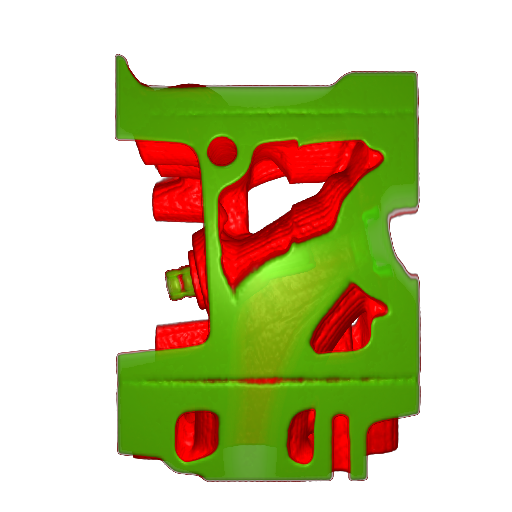
\includegraphics[width=1\linewidth]{images/engine_naive}
		\subcaption{$ P $}
	\end{minipage}~
	\begin{minipage}{.33\textwidth}
		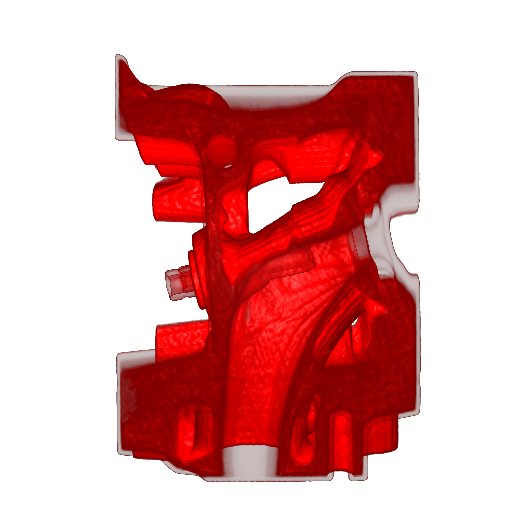
\includegraphics[width=1\linewidth]{images/engine_naive_1}
		\subcaption{$ P_{1} $}
	\end{minipage}~
	\begin{minipage}{.33\textwidth}
		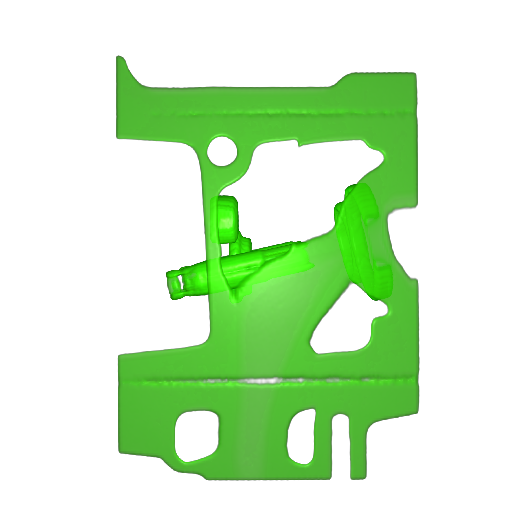
\includegraphics[width=1\linewidth]{images/engine_naive_2}
		\subcaption{$ P_{2} $}
	\end{minipage}
	\caption{(a) An engine block; (b) and (c) isolated volume rendering images of the red feature and the green feature}
	\label{fig:engine_naive}
\end{figure}

\begin{figure}
	\centering
	\begin{minipage}{.33\textwidth}
		
\includegraphics[width=1\linewidth]{images/engine_naive_saliencemap}
		\subcaption{$ S $}
	\end{minipage}~
	\begin{minipage}{.33\textwidth}
		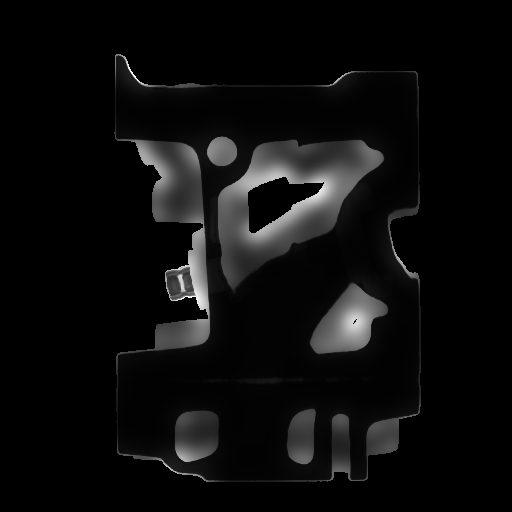
\includegraphics[width=1\linewidth]{images/engine_naive_saliencemap_1_overlap}
		\subcaption{$ S_{1} $}
	\end{minipage}~
	\begin{minipage}{.33\textwidth}
		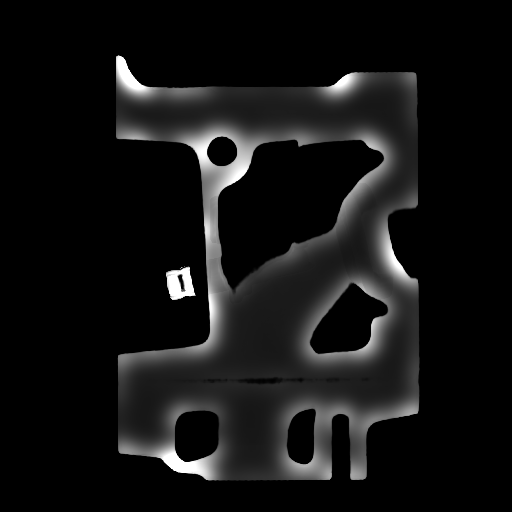
\includegraphics[width=1\linewidth]{images/engine_naive_saliencemap_2_overlap}
		\subcaption{$ S_{2} $}
	\end{minipage}
	\caption{(a) The 2D saliency map; (b) and (c) the feature saliency maps of the two features. The saliency maps are enhanced (multiplied by 8) for better contrast in illustrations.}
	\label{fig:engine_naive_saliencemap}
\end{figure}

\begin{figure}
	\centering
	\begin{minipage}{.33\textwidth}
		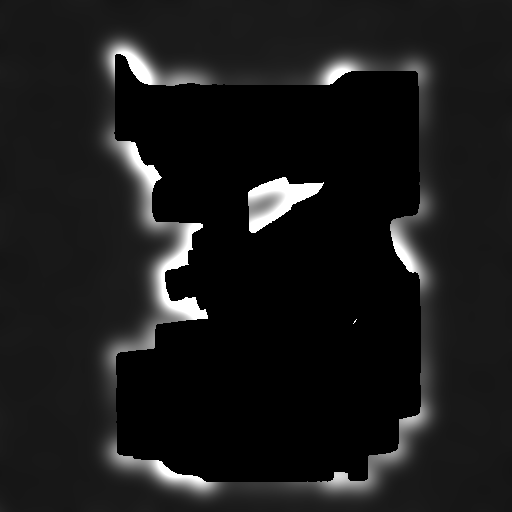
\includegraphics[width=1\linewidth]{images/engine_naive_saliencemap_left}
		\subcaption{$ S' $}
	\end{minipage}~
	\begin{minipage}{.33\textwidth}
		
\includegraphics[width=1\linewidth]{images/engine_naive_gaussian_1}
		\subcaption{$ G_{1} $}
	\end{minipage}~
	\begin{minipage}{.33\textwidth}
		
\includegraphics[width=1\linewidth]{images/engine_naive_gaussian_2}
		\subcaption{$ G_{2} $}
	\end{minipage}
	\caption{(a) The residual saliency image; (b) and (c) the Gaussians of the two feature saliency maps with a kernel size of one eighth of the image width}
	\label{fig:engine_naive_saliencemap_left}
\end{figure}

\begin{figure}
	\centering
	\begin{minipage}{.33\textwidth}
		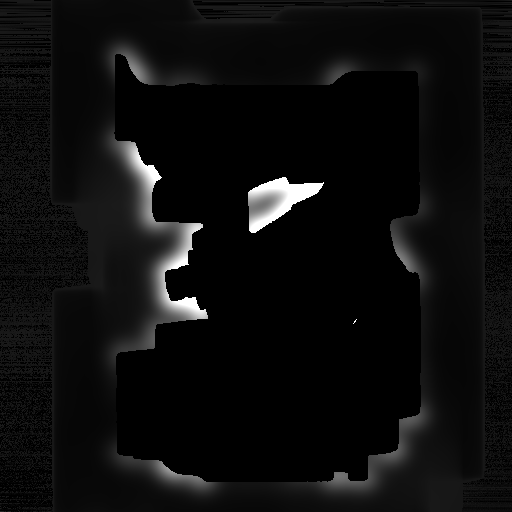
\includegraphics[width=1\linewidth]{images/engine_naive_leftgaussian_1}
		\subcaption{$ S'_{1} $}
	\end{minipage}~
	\begin{minipage}{.33\textwidth}
		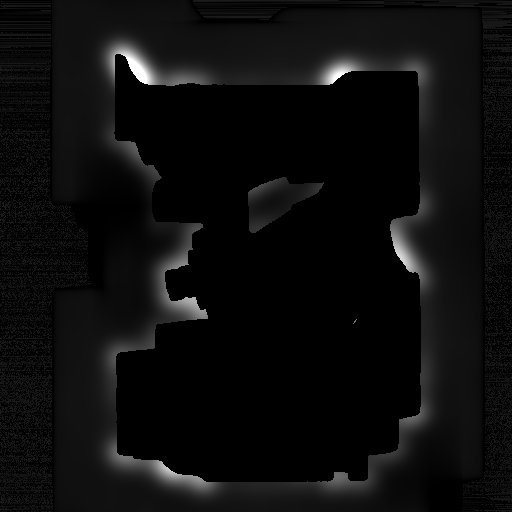
\includegraphics[width=1\linewidth]{images/engine_naive_leftgaussian_2}
		\subcaption{$ S'_{2} $}
	\end{minipage}
	\caption{The residual saliency images of the two features}
	\label{fig:engine_naive_leftgaussian}
\end{figure}

\begin{figure}
	\centering
	\begin{minipage}{.33\textwidth}
		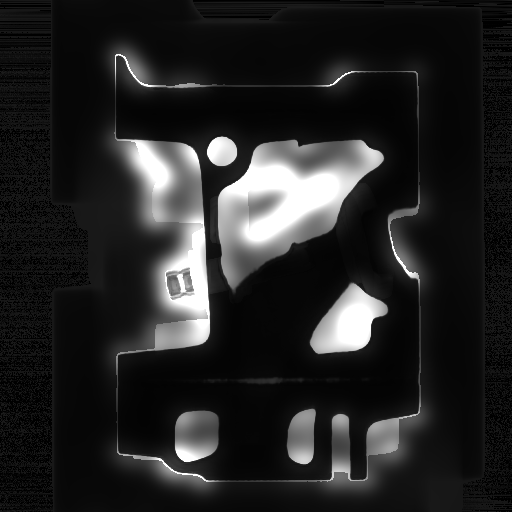
\includegraphics[width=1\linewidth]{images/engine_naive_saliencemap_1}
		\subcaption{$ T_{1} $}
	\end{minipage}~
	\begin{minipage}{.33\textwidth}
		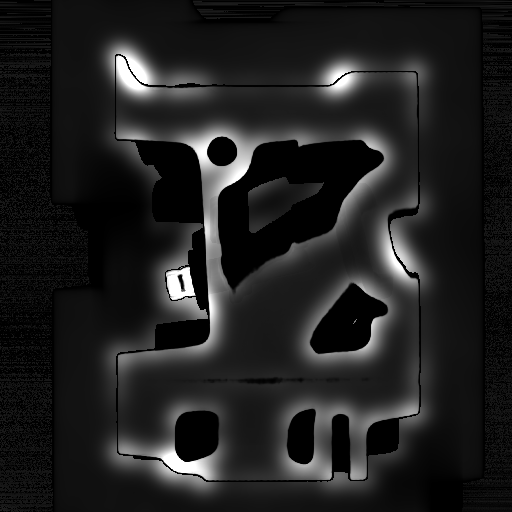
\includegraphics[width=1\linewidth]{images/engine_naive_saliencemap_2}
		\subcaption{$ T_{2} $}
	\end{minipage}~
	\begin{minipage}{.33\textwidth}
		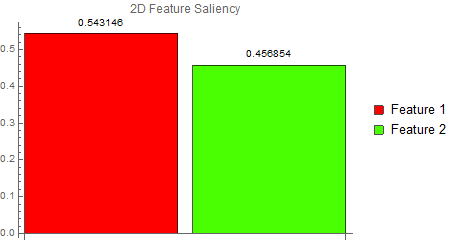
\includegraphics[width=1\linewidth]{images/engine_naive_2DFS}
		\subcaption{2D feature saliency}
	\end{minipage}
	\caption{(a) and (b) The total feature saliency maps of the two features; (c) 2D feature saliency of the two features}
	\label{fig:engine_naive_saliencemap_features}
\end{figure}

%% \chapter{Experiment Questionnaire \label{Experiment_pdf}}

This is the questionnaire used in the experiment presented in Section~\ref{experiment_section}.

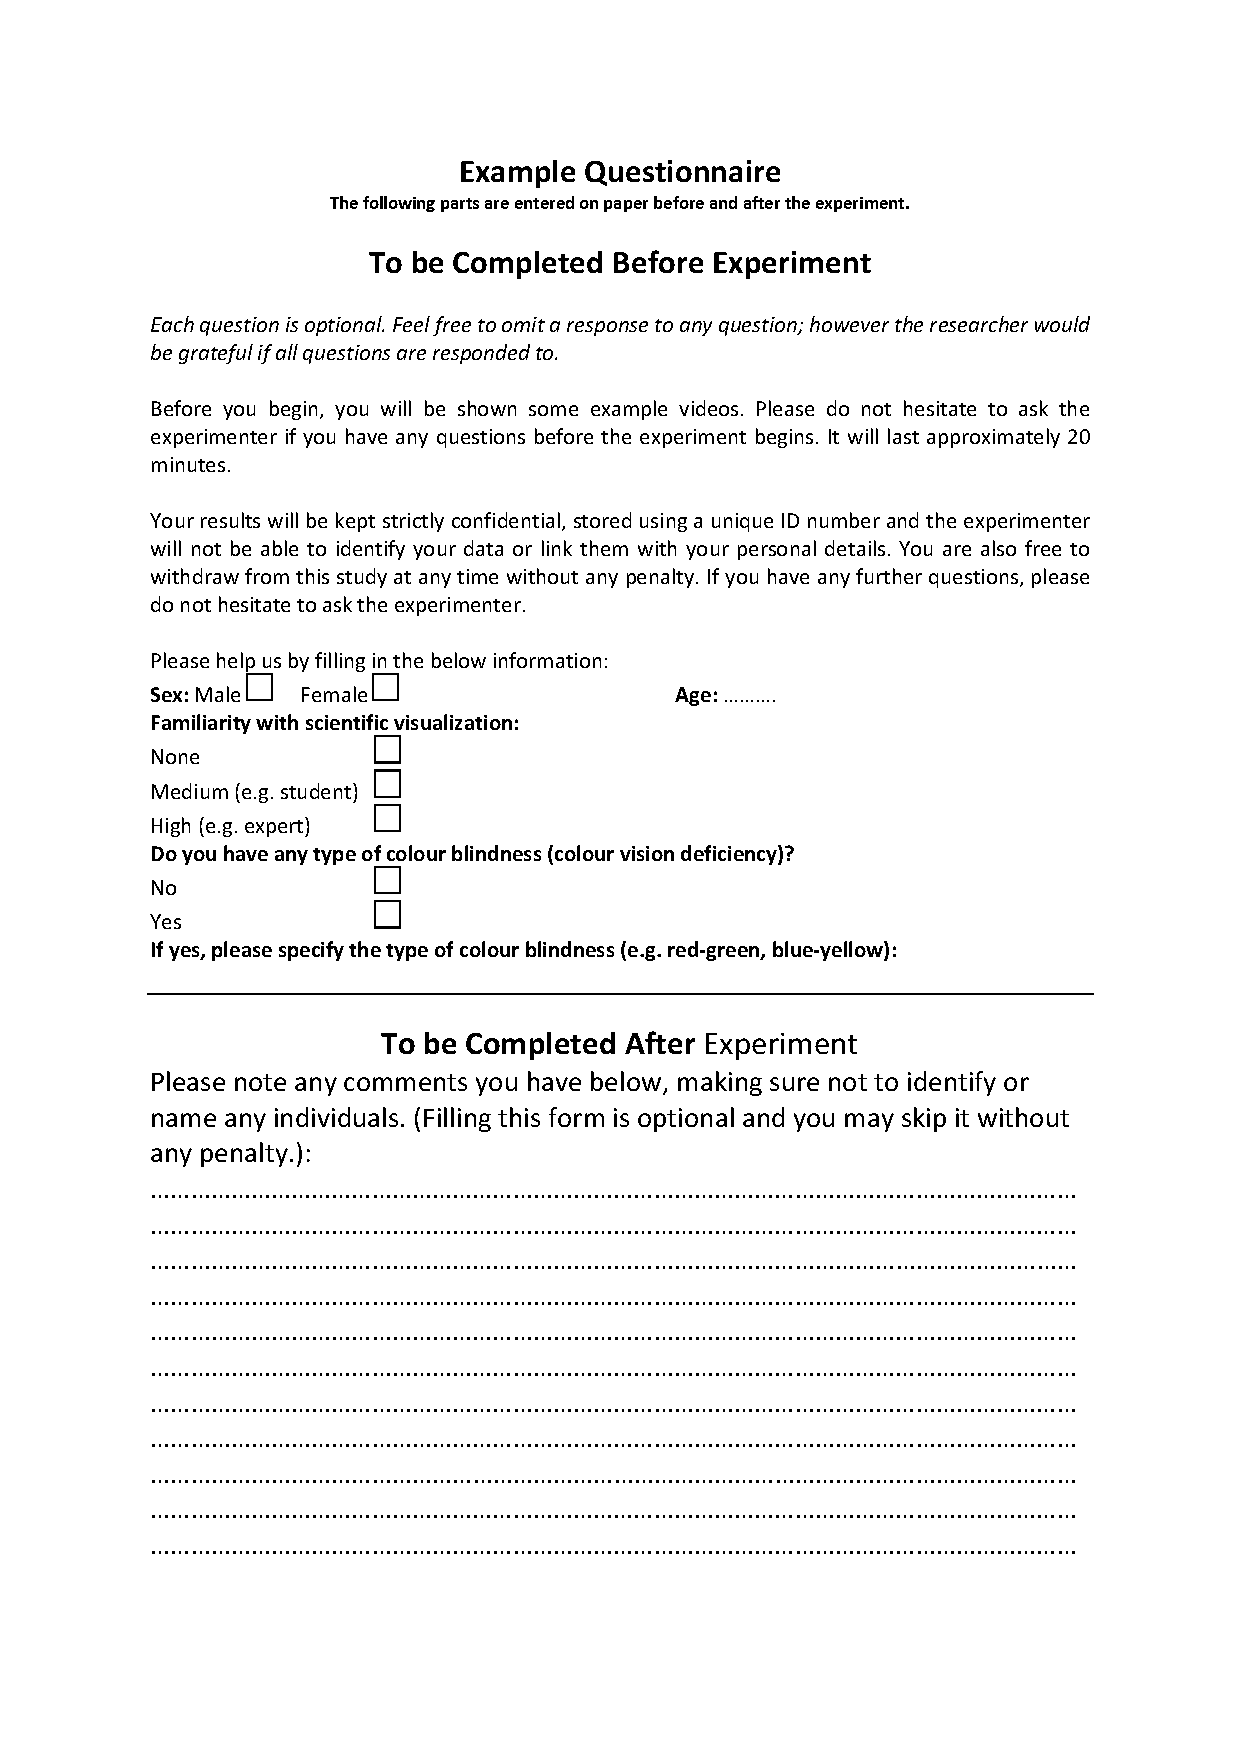
\includepdf[pages={-}]{Questionnaire_real.pdf}

%\end{appendix}


%\addcontentsline {toc}{chapter}{Bibliography}     %% Force Bibliography to appear in contents

%\begin{thebibliography}{ieeetr}                   %% Start your bibliography here; you can
%%\bibliography{refs}                               %% also use the \bibliography command
%\end{thebibliography}                             %% to generate your bibliography.

%%%%%%%%%%%%%%%%%%%%%%%%%%%%%%%%%%%%%%%%%%%%%%%%%%%%%%%%%%%%%
%% BIBLIOGRAPHY AND OTHER LISTS
%%%%%%%%%%%%%%%%%%%%%%%%%%%%%%%%%%%%%%%%%%%%%%%%%%%%%%%%%%%%%
\bibliographystyle{ieeetr}
\bibliography{bibliography}

\end{document}                                    %% END THE DOCUMENT
